\documentclass[tikz,border=3mm]{standalone}
\usepackage{pgfplots}
\begin{document}

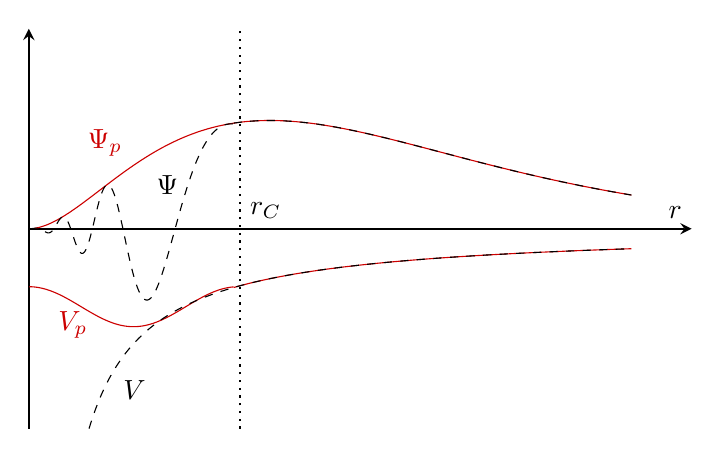
\begin{tikzpicture}
    \begin{axis}[
            domain=0.01:1,
            xmin=0, xmax=1.1,
            ymin=-1, ymax=1,
            samples=400,
            axis y line=center,
            axis x line=middle,
            ticks=none,
            axis line style = thick,
            xlabel=$r$,
            width=10cm,
            height=6.66cm
        ]
        \addplot+[mark=none, thick, dotted, color=black] coordinates {(0.35, -1) (0.35,1)} node[above right, pos=0.5] {$r_C$};
        \addplot+[mark=none, domain=0.001:0.34, color=red!80!black] {0.1*cos(330*3.14*x)-0.39} node[below, pos=0.2] {$V_p$};
        \addplot+[mark=none, domain=0.34:1, color=red!80!black] {-0.1/x};
        \addplot+[mark=none, color=red!80!black] {(5*x)^2*e^(-5*x)} node[above left, pos=0.25] {$\Psi_p$};
        \addplot+[mark=none, domain=0.001:0.34, dashed, color=black] {(5*x)^2*e^(-5*x)*sin(400*3.14*e^(-8*x))} node[left, pos=0.85] {$\Psi$};
        \addplot+[mark=none, domain=0.34:1, dashed, color=black] {(5*x)^2*e^(-5*x)};
        \addplot+[mark=none, domain=0.1:1, dashed, color=black] {-0.1/x} node[below right, pos=0.2] {$V$};



    \end{axis}
\end{tikzpicture}
\end{document}
